\documentclass [a4paper, 12pt]{article}

\usepackage[warn]{mathtext} 		% русские буквы в фомулах
\usepackage[T2A]{fontenc}			% кодировка
\usepackage[utf8]{inputenc}			% кодировка исходного текста
\usepackage[english,russian]{babel}	% локализация и переносы
\usepackage{cmap}					% поиск в PDF
\usepackage{tikz}
\usepackage{pgfplots}

%%% Нормальное размещение таблиц (писать [H] в окружении таблицы)
\usepackage{float}
\restylefloat{table}


% Математика
\usepackage{amsmath,amsfonts,amssymb,amsthm,mathtools} 


\usepackage{wasysym}


%Заговолок
\title{Отчёт о выполнении лабораторной работы №3.5.1 \\ {Изучение плазмы газового разряда в неоне.}}
\author{Устюжанина Мария, Б01-107, ФРКТ}


\begin{document}

\maketitle
\newpage

\section{Аннотация}

    
    \textbf{Цель работы:} изучение вольт-амперной характеристики тлеющего разряда; изучение свойств плазмы методом зондовых характеристик.
    
    \textbf{В работе используются:} стеклянная газоразрядная трубка, наполненная неоном; высоковольтный источник питания; источник питания постоянного тока; делитель напряжения; потенциометр; амперметры; вольтметры; переключатели.




%----------------------------------------------------
\section{Теоретические сведения и методика измерений}

    \textbf{Тлеющий разряд} -- электрический разряд в газе низекого давлнеия.
 
    \textbf{Свечение плазмы} -- следствие непрерывно идущей рекомбинации электронов и ионов в нейтральные атомы при относительно невысоких температурах. В этом процессе выделяется энергия и уменьшаеься концентрация электронов и ионов. В тлеющем газовом разряде обычно: <<горячие>> элктроны и <<холодные>> ионы: $T_e > > T_i$, так как масса электрона много меньше массы иона $m_e < < m_i$,следовательно, электроны ускоряются внешним полем почти без потерь энергии, а иону быстро отдают энергию от поля и электронов нейтральным атомам газа и стенкам сосуда.

\subsection*{Дебаевский радиус}

    Плазменные колебания могут быть возбуждены как за счёт внешнего воздействия (например, при прохождении электромагнитной волны), так и за счёт тепловой энергии, содержащейся непосредственно в плазме. Оценим амплитуду колебаний в последнем случае. Средняя скорость теплового движения электронов по порядку величины равна

\[ \bar{v_e} \sim \sqrt{\frac{K_{Б}T_e}{m_e}}\]

    где $T_e$ -- температура электронов. Амплитуду $r$ колебаний электронов относительно ионов оценим как смещение с тепловой скоростью $\bar{v_e}$ за характерное время плазменных колебаний $\frac{1}{w_p}: r = \frac{\bar{v_e}}{w_p}$. Зная, что $w_p = \sqrt{\frac{4\pin_e e^2}{m_e}}$, получим:
    
\[r_D = \sqrt{\frac{k_{Б}T_e}{4\pi n_e e^2}} \sim \frac{v_e}{w_p}\]

    Эту величину называют \textbf{дебаевским радиусом} (дебаевской длиной). Из рассмотренного примера видно, что дебаевская длина есть амплитуда ленгмюровских колебаний, возбуждаемых тепловыми флуктуациями. Она задаёт масштаб, на котором возможно спонтанное нарушение квазинейтральности плазмы.

    Таким образом, плазменная частота $w_p$ и дебаевская длина $r_D$ определят временную и пространственную масштабы коллективного движения электронов относительно ионов.


\subsection*{Плазменная частота}

\begin{center}
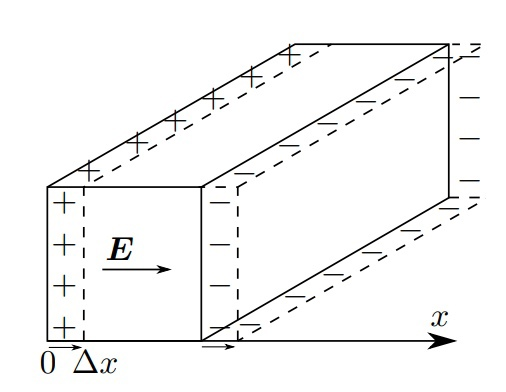
\includegraphics[width=5cm, height=4cm]{plch_351.jpg}
\end{center}
\begin{flushright}
{\small \textbf{Рис. 1.} \text {Плазменные колебания}}
\end{flushright}

    Теперь выделим параллелепипед с плотностью $n$ электронов, сместим их на $x$. Возникнут поверхностные заряды плотностью $\sigma = nex$, поле от которых $E = 4\pin_e \Delta x$ будет придавать электронам ускорение:
    
\[
\dfrac{d^2x}{dt^2}=-\dfrac{eE}{m}=-\dfrac{4\pi n e^2}{m}
\]

    откуда получаем уравнение гармонических колебаний:
    
\[\Ddot{\Delta x} + \frac{4 \pi n_e e^2}{m} \Delta x = 0 \]


    Следовательно, \textbf{плазменная (ленгмюровская) частота} колебаний электронов:
    
\begin{equation}
\omega_p = \sqrt{\dfrac{4\pi ne^2}{m}}.
\end{equation}

    Нами получен один из важнейших параметров плазмы. Плазменная частота определяет характрный временной масштаб плазы - время отклика на флуктуацию плотности заряда в ней. Часот аопределяет многие физические процессы, включая распространение электромагнитных волн в плазме.


\subsection*{Равновесная и неравновесная плазма}

    \textbf{Равновесная плазма} - плазма, в которой в состоянии теплового равновесия все частицы (электроны, ионы, нейтральные) имеют максвелловское распределение по скоростям, а их температуры равны: $T_e = T_i = T_n$.
    При тепловом равновесии с окружающей средой равновесная плазма может существовать неограниченно долго.

    \textbf{Неавновесная плазма} - плазма, в которой имеет место разделение температур компонентов, образующих её. При прекращении действия внешних источников неравновесная плазма исчезает в течение малых долей секунды ($\sim 10^{-5} - 10^{-4}$).


    В нашем эксперименте плазма является неравновесной.






%------------------------------------------------
\section{Экспериментальная установка}


\begin{center}
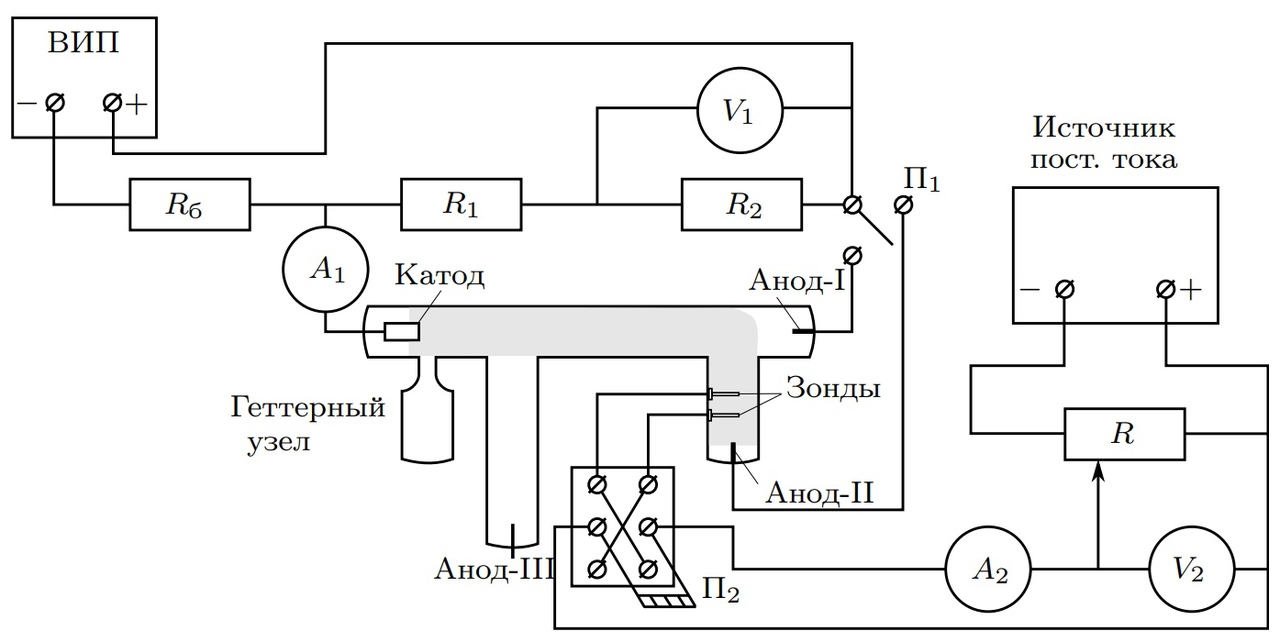
\includegraphics[width=12cm, height=6cm]{sheme_351.jpg}
\end{center}
\begin{flushright}
{\small \textbf{Рис. 2.} \text {Экспериментальная установка}}
\end{flushright}

    Параметры нашей установки:

\begin{itemize}
    \item Давление в трубке = 2 мм рт. ст.
    \item $d = 0,2 мм$
    \item $l = 5,2 мм$
\end{itemize}




    
%------------------------------------------------
\section{Результаты измерений и обработка данных}

%-----------------------------------------
\subsection{Вольт-амперная характеристика}

    Построим вольт-амперную характеристику разряда в координатах $I_p(U_p)$. По наклону кривой определим максимальное дифференциальное сопротивление разряда $R_{дифф}$

\begin{center}
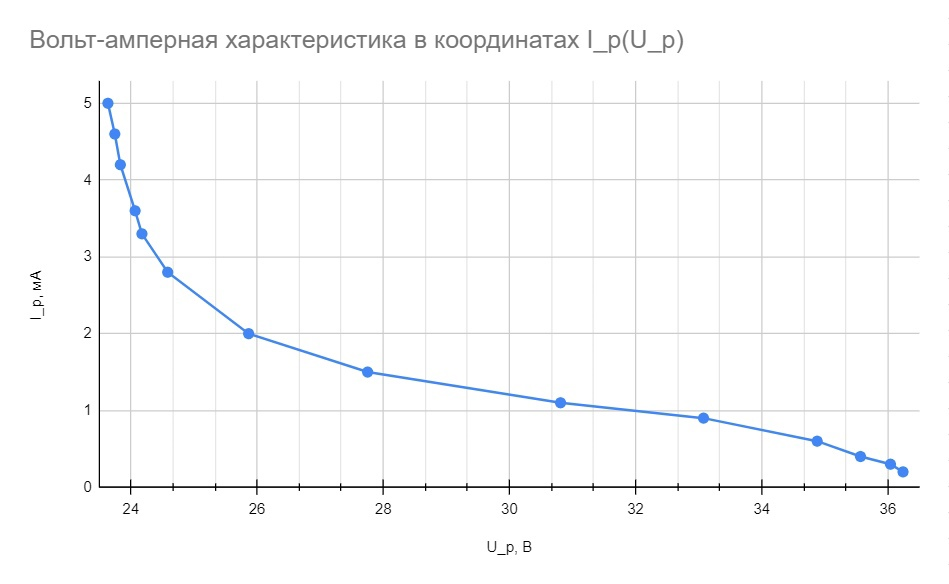
\includegraphics[width=12cm, height=8cm]{vax_351.jpg}
\end{center}
\begin{flushright}
{\small \textbf{Рис. 3.} \text {Вольт-амперная характеристика разряда}}
\end{flushright}

\[R_{дифф} = \frac{dU}{dI} = \frac{24,66}{2} = 12,33\]

    Полученная нами часть вольт-амперной характеристики соответствует участку ДГ ВАХ разряда в неоне при давлении  1 тор (см. Рис.4).

\begin{center}
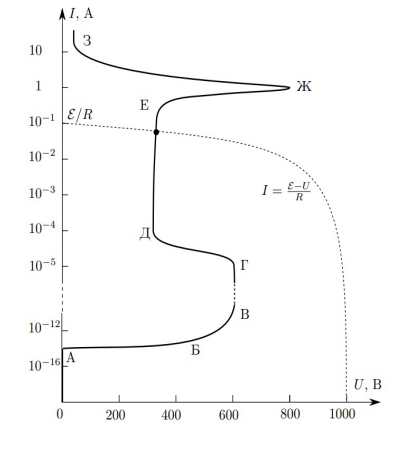
\includegraphics[width=6cm, height=7cm]{vax 351.jpg}
\end{center}
\begin{flushright}
{\small \textbf{Рис. 4.} \text {Вольт-амперная характеристика разряда в неоне при давлении  1 тор.}}
\end{flushright}   


%-----------------------------------
\subsection{Зондовые характеристики}

    Построим зондовые характеристики $I(U)$ для трех токов: $I_1 = 5 A, I_2 = 3 A, I_3 = 0,5 A$. Рассчитаем для каждого тока ионный ток насыщения $I_{in}$, наклон характеристики в начале координат $\frac{dI}{dU}$, температуры электронов $T_e$, концентрации электронов и ионов в плазме $n_e, n_i$ ($S = \pi d l$). Полученные формулы представлены в таблице 1.


    
\begin{center}
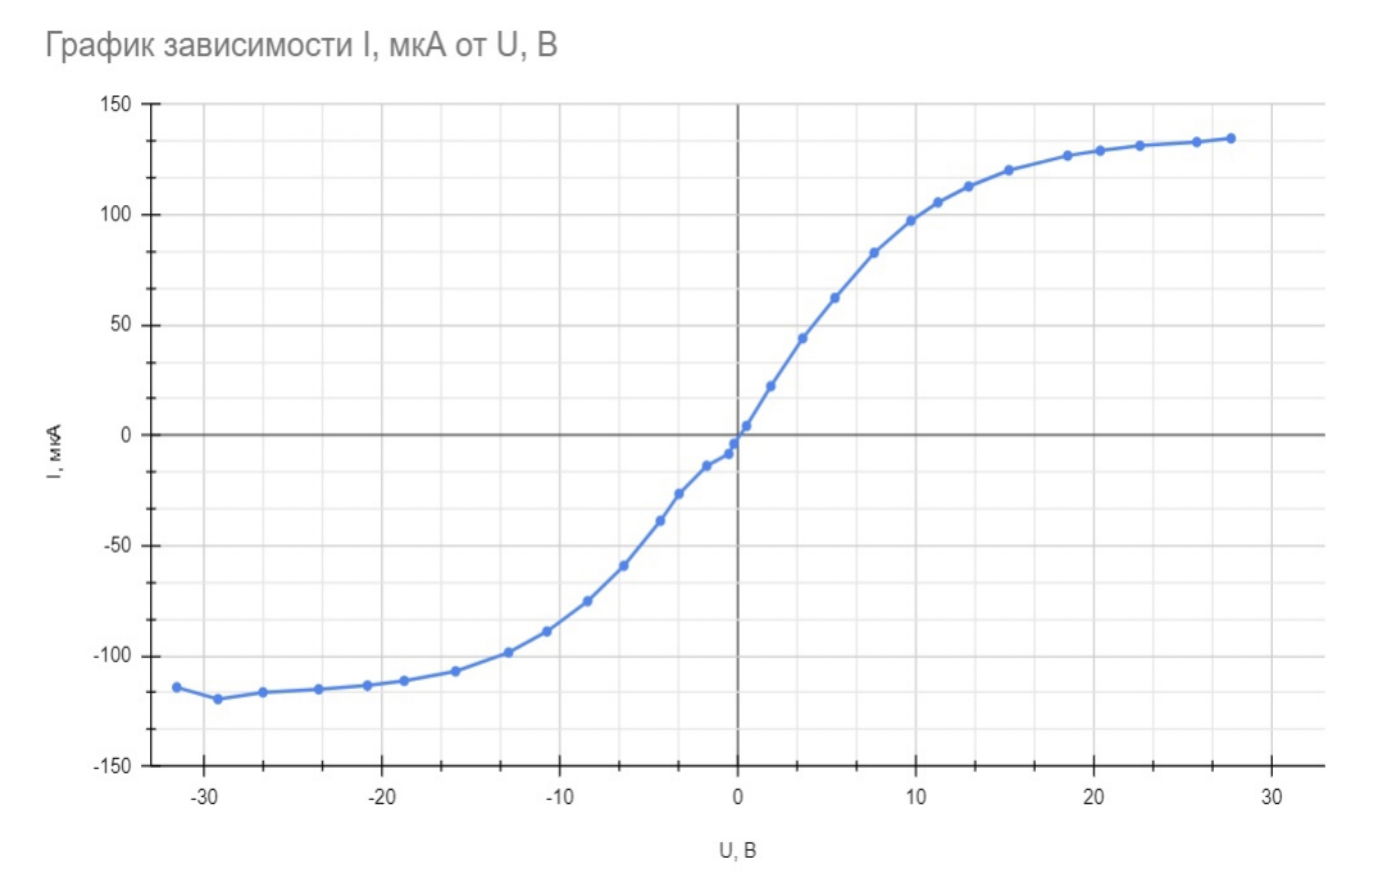
\includegraphics[width=12cm, height=8cm]{Py2_351.jpg}
\end{center}
\begin{flushright}
{\small \textbf{Рис. 4.} \text {Зондовая характеристика при $I = 5 A$}}
\end{flushright}
\begin{center}
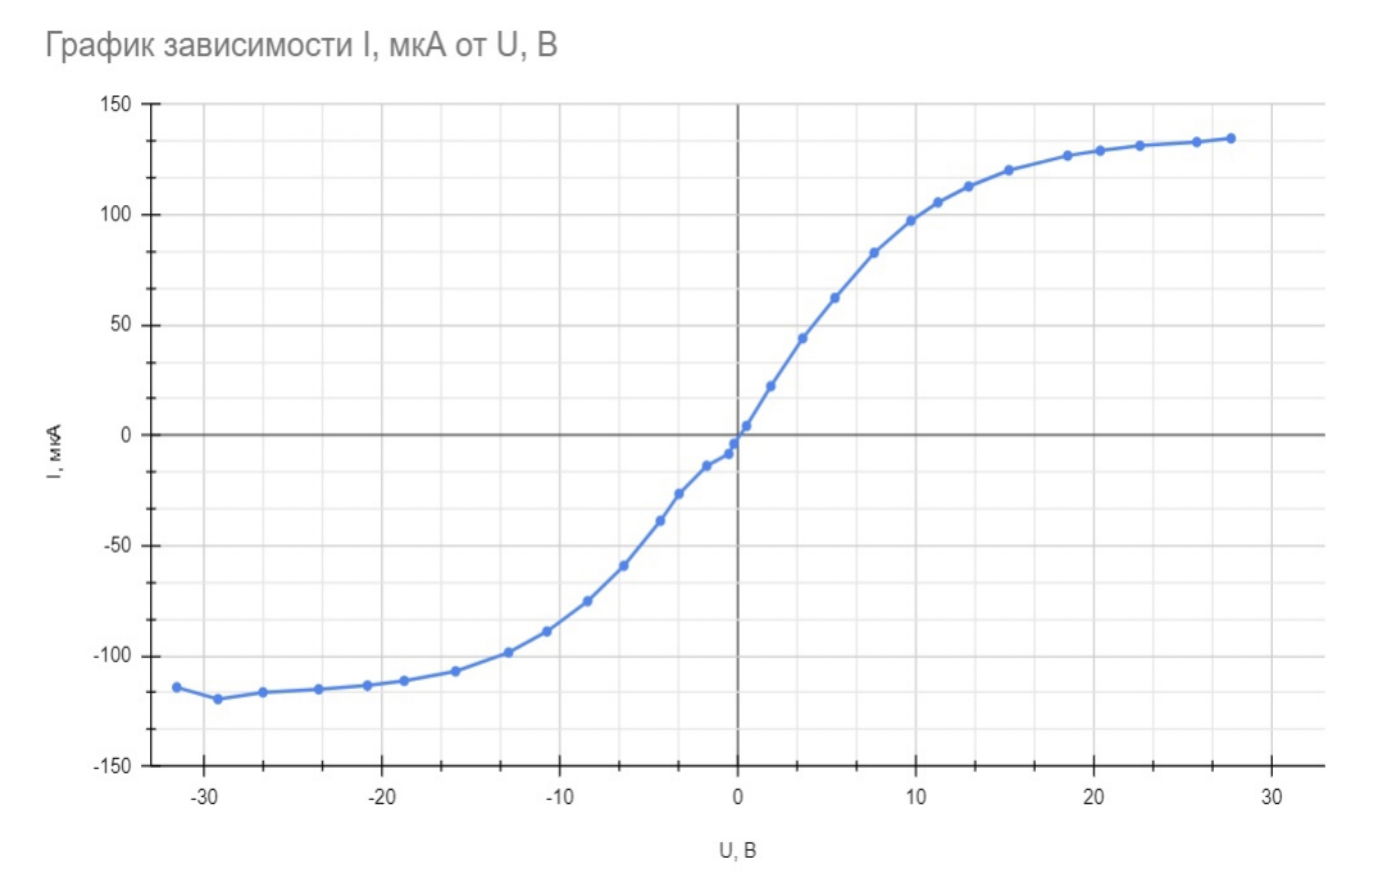
\includegraphics[width=12cm, height=8cm]{Py2_351.jpg}
\end{center}
\begin{flushright}
{\small \textbf{Рис. 5.} \text {Зондовая характеристика при $I = 3 A$}}
\end{flushright}
\begin{center}
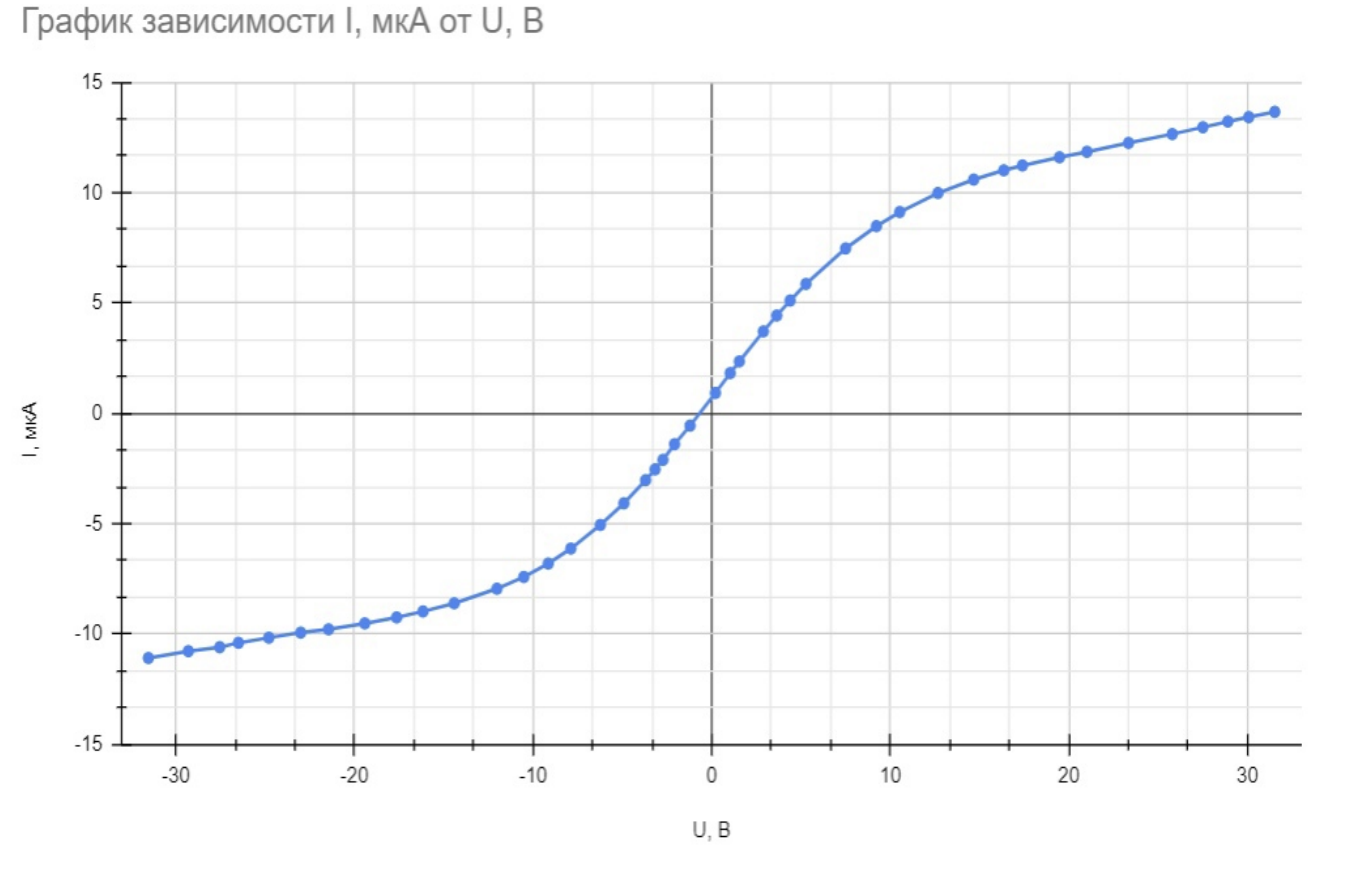
\includegraphics[width=12cm, height=8cm]{Py1_351.jpg}
\end{center}
\begin{flushright}
{\small \textbf{Рис. 6.} \text {Зондовая характеристика при $I = 0.5 A$}}
\end{flushright}


\begin{table}[]
\centering
\begin{tabular}{|l|l|l|l|l|l|}
\hline
I, мА & $I_{in}$, мкА & $dI/dU$ & $T_e$, K & $n_i м^{-3}$ & $n_e м^{-3}$ \\ \hline
5 & 110 & $1,07\cdot10^{-5}$ & 37192,8 & $7,5\cdot10^{16}$ & $8,2\cdot10^{16}$ \\ \hline
3 & 60 & $7,08\cdot10^{-6}$ & 30689,8 &  $4,5\cdot10^{16}$ & $5,3\cdot10^{16}$ \\ \hline
0,5 & 8 & $9,8\cdot10^{-7}$ & 29676,9 & $6,12\cdot10^{15} $ & $8,0\cdot10^{15}$b \\ \hline
\end{tabular}
\end{table}

\begin{table}[]
\centering
\begin{tabular}{|l|l|l|}
\hline
$\omega_p, 1/с$ & $r_{D_е}, 10^{-3} см$ & $N_D$\\ \hline
171212,8 & 5,5 & 53754,1 \\ \hline
136542,9 & 6,3 & 47698,8 \\ \hline
53098,12 & 16,0 & 104578,04 \\ \hline
\end{tabular}
\end{table}

\begin{flushright}
{\small \textbf{Табл. 1.} \text {Результат.}}
\end{flushright}


\begin{center}
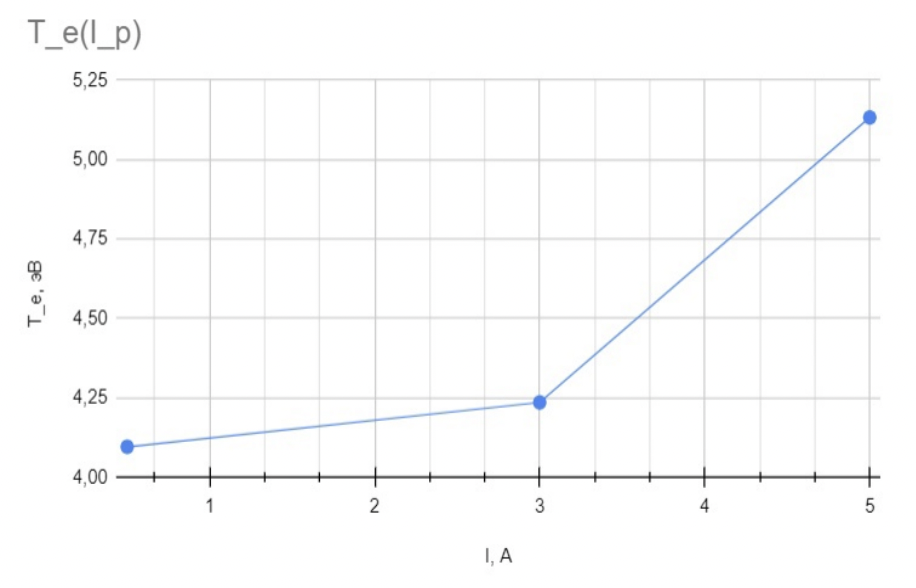
\includegraphics[width=12cm, height=8cm]{ris7.jpg}
\end{center}
\begin{flushright}
{\small \textbf{Рис. 7.} \text {График зависимости $T_e(I_p)$}}
\end{flushright}

\begin{center}
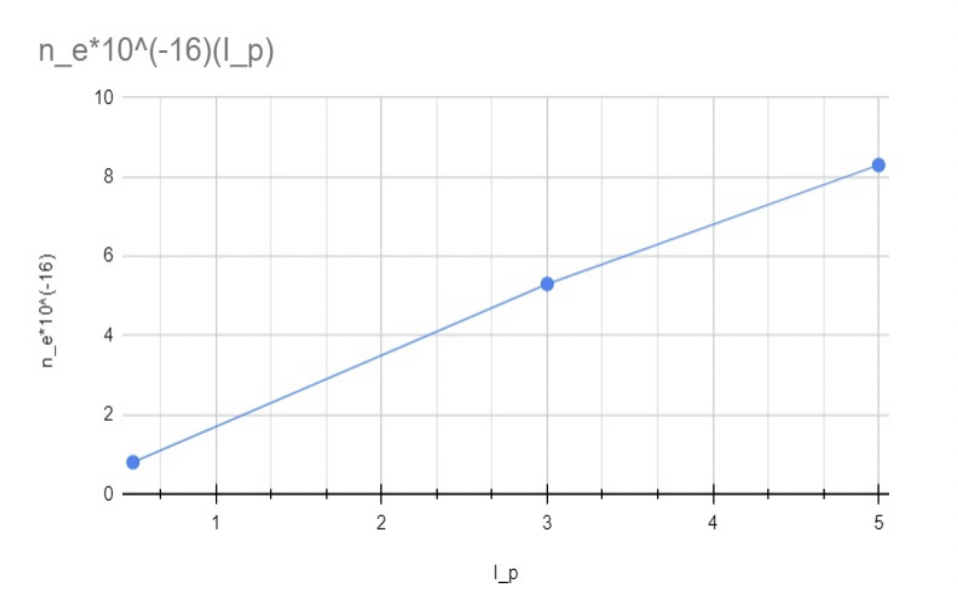
\includegraphics[width=12cm, height=8cm]{ris8.jpg}
\end{center}
\begin{flushright}
{\small \textbf{Рис. 8.} \text {График зависимости $n_e(I_p)$}}
\end{flushright}

\section{Выводы}
\begin{enumerate}
    \item В этой работе мы изучили ВАХ тлеющего разряда.
    \item А затем изучениои свойств плазмы методом зондовых характеристик. Мы получили температуру электронов,
    Концентрация электронов в плазме получилвсь порядка \(10^18\; m^{-3}\).
    Плазменная частота колебаний \(\omega \simeq 10^6 rad/sec\).
    Дебаевский радиус порядка \(10^{-3}\; m\) и число ионов в нём много больше единицы.


\end{document}
